%\VignetteIndexEntry{Introduction to SpaDES: A package to develop and run spatially explicit discrete event simulation models.}
%\VignetteDepends{SpaDES}
%\VignetteKeyword{discrete event simulation}
\documentclass{article}

%%% latex packages
\usepackage[T1]{fontenc}
\usepackage{hyperref}
\usepackage[utf8]{inputenc}
\usepackage[usenames,dvipsnames]{xcolor}

%% change margins to 1" all the way around
\oddsidemargin 0.0in
\evensidemargin 0.0in
\textwidth 6.5in
\headheight 0.0in
\topmargin 0.0in
\textheight 9.0in

%%% document info
\title{Introduction to \texttt{SpaDES}}

\author{
  Alex M. Chubaty\\
	\small{Natural Resources Canada, Pacific Forestry Centre}\\
	\small{email: \href{mailto:achubaty@nrcan.gc.ca}{achubaty@nrcan.gc.ca}}
	\and
	Eliot McIntire\\
	\small{Natural Resources Canada, Pacific Forestry Centre}\\
	\small{email: \href{mailto:emcintir@nrcan.gc.ca}{emcintir@nrcan.gc.ca}}
}

\usepackage{Sweave}
\begin{document}
\Sconcordance{concordance:introduction.tex:introduction.Rnw:%
1 31 1 1 0 14 1 1 3 2 0 1 1 1 10 8 0 1 2 7 0 1 5 14 1 1 2 1 0 4 1 1 2 4 %
0 1 2 22 1 1 2 1 0 1 4 2 0 1 2 1 0 3 1 1 5 3 0 1 1 1 2 11 0 1 1 15 0 1 %
7 5 0 1 2 5 0 1 2 7 1}

 % displays code as entered (no arranging lines)

\maketitle

\abstract{Implement a variety of simulation models, with a focus on spatially explicit raster models and agent based models. The core simulation components are built upon a discrete event simulation framework that facilitates modularity, and enables the user to include additional functionality by running user-built simulation modules. Included are numerous tools to visualize raster and other maps.\\
\\
\textbf{Website:} \url{https://github.com/achubaty/SpaDES}}

\tableofcontents

\newpage

\section{Introduction}

\subsection{Objectives and motivations}

\paragraph{}
Building spatial simulation models often involves reusing various components, often having to reimplement similar fuctionality in multiple simulation frameworks (i.e, in different programming languages). When various components of a simulaiton model become fragmented across multiple platforms, it becomes increasingly difficult to link these various components, and often solutions for this problem are idiosyncratic and specfic to the model being implemented.

\paragraph{}
\texttt{SpaDES} is a generic simulation platform that can be used to create new model components quickly. It also provides a framework to link with existing simulation models, so that an already well described and mature model, \textit{i.e.}, Landis-II, can be used with \textit{de novo} components. Alternatively one could use several \textit{de novo} models and several existing models in combination. This approach requires a platform that allows for modular reuse of model components (herein called ``modules'') as hypotheses that can be evaluated and tested in various ways.

\paragraph{}
When beginning development of this package, we sought a general simulation platform at least the following characteristics:

\begin{enumerate}
  \item Allow rapid building of models of a wide diversity of types (IBMs, raster models, differential equation models, etc.);
  \item Run faster and more memory efficiently than current systems for doing similar things (NetLogo, SELES, Repast, etc.),
  \item Use a platform that already has strong data analysis and manipulation capacities;
  \item Be open source, but also make it as easy as possible for many people to easily contribute modules and code;
  \item Be easy to use for a large number of scientists who aren't formally trained as computer programmers;
  \item Should be built around modularity so that models can be seen as modules that are easily replaceable, not just ``in theory'' replaceable;
  \item Allow tight coupling between data and model simulations so that calibration is not actually something that one has to redesign every time there is a new data set.
\end{enumerate}

\paragraph{}
We selected\textsf{R} as the system within which to build \texttt{SpaDES}. \textsf{R} is currently the \textit{lingua franca} for scientific data analysis. This means that anything developed in \texttt{SpaDES} is simply \textsf{R} code and can be easily shared with journals and the scientific community. We can likewise leverage \textsf{R}'s strengths as a data platform, its capabilities to run external code such as C and Python, call external software such as databases, its excellent visualization and graphics, and its abilities for high performance computing. We don't have to implement all of these from scratch ourselves!

\subsection{Discrete event simulation and \texttt{SpaDES}}

\paragraph{}
Discrete event simulation (DES) as implement here is ``event driven'', meaning that an activity changes the state of the system at particluar times (called events). This approach assumes that state of the system only changes due to events, therefore there is no change between events. A particular activity may have several events associated with it. Future events are scheduled in an event queue, and then processed in chronological order.  Because the system state doesn't change between events, we do not need to `run the clock' in fixed increments each timestep. Rather, time advances to the time of the next event in the queue.

\paragraph{}
`Time' is the core concept linking various simulation components via the event queue. Activities schedule events (which change the system according to their programmed rules) and do not need to know about each other. This allows for modularity of simulation components. Thus, complex simulations involving multiple processes (activities) can be built fairly easily, provided these processes are modelled using a common DES framework.

\paragraph{}
\texttt{SpaDES} provides such a framework, facilitating interaction between multiple processes (built as ``modules'') that don't interact with one another directly, but are scheduled in the event queue and carry out operations on shared data objects in the global simulation environment. This package provides tools for building modules natively in \textsf{R} that can be reused. Additionally, because of the flexibility\textsf{R} provides for interacting with other programming languages and external data sources, modules can also be built using external tools and integrated with \texttt{SpaDES} (see Figure \ref{figure-SpaDES-overview}).

\begin{figure}[!htbp]
  \centering
	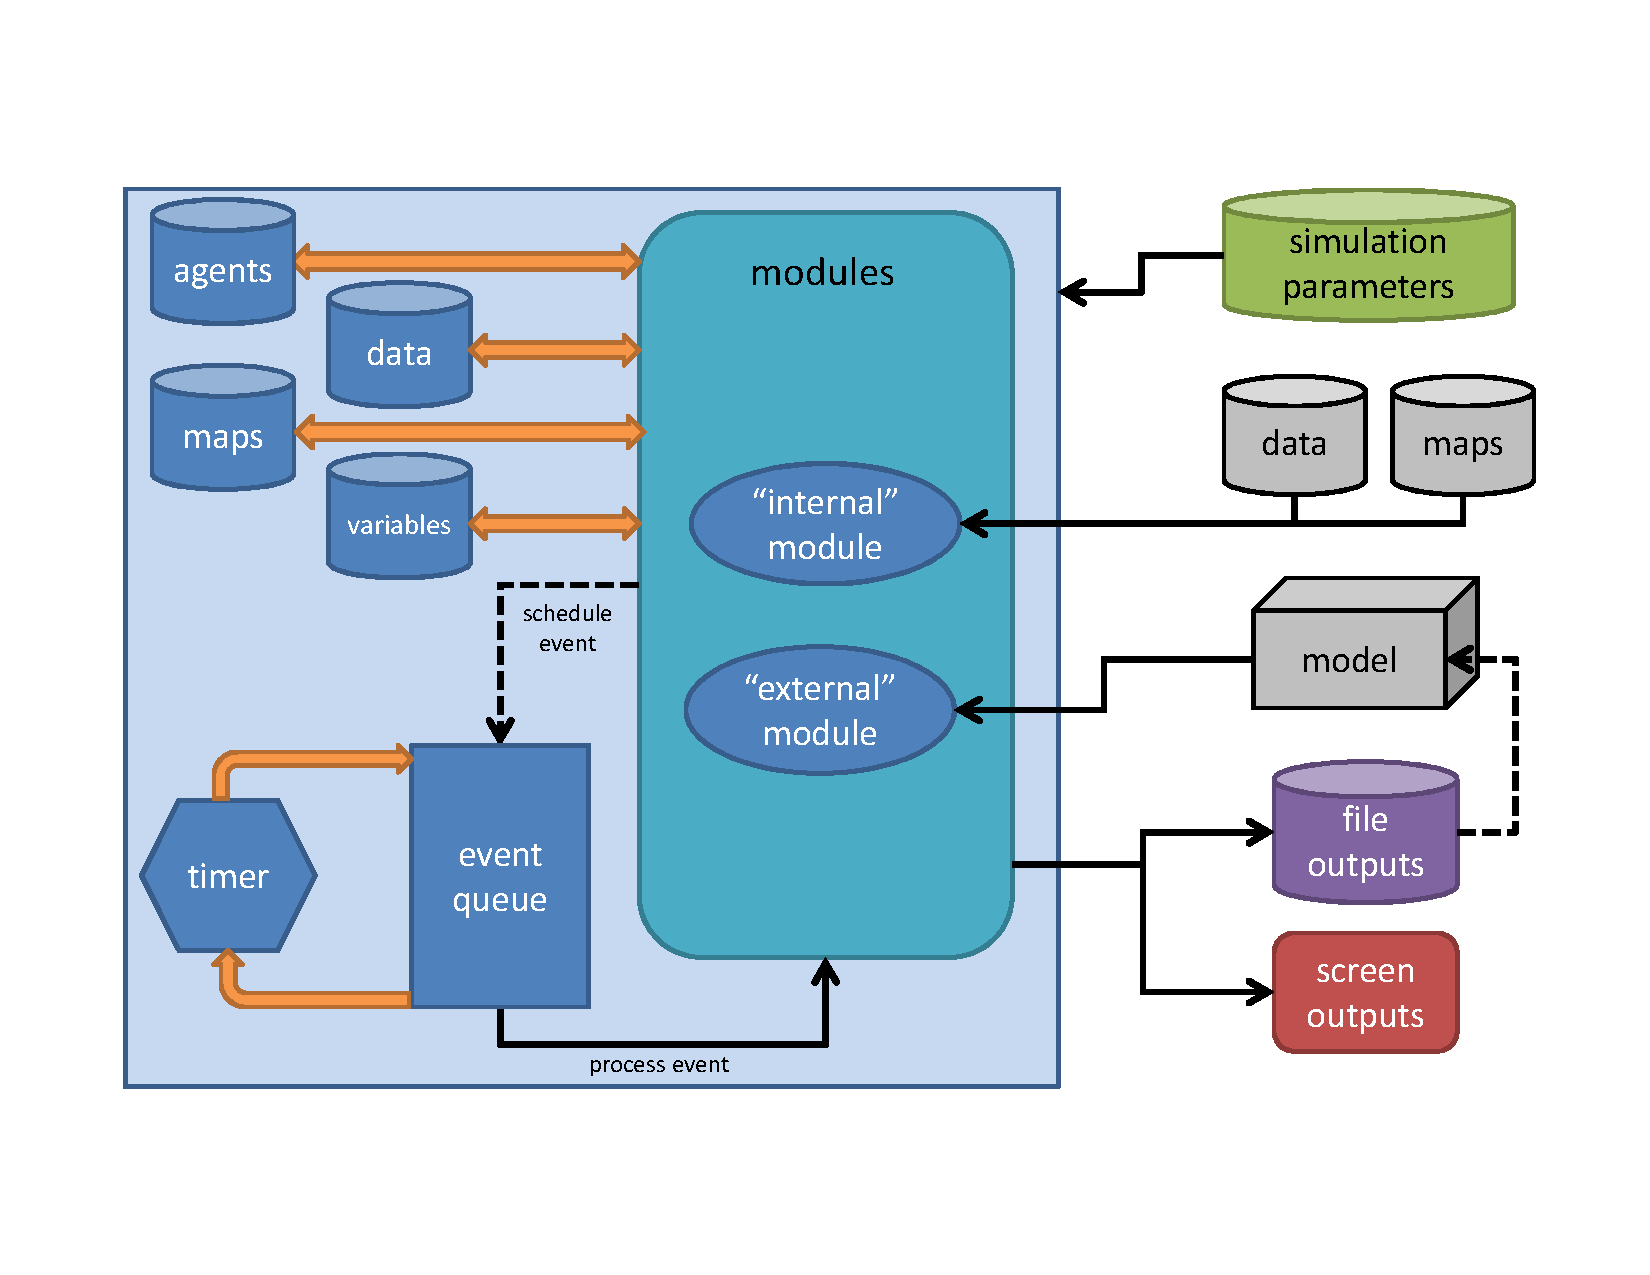
\includegraphics[width=5in]{../inst/SpaDES-overview-diagram.pdf}
	\caption{Schematic representation of a \texttt{SpaDES} simulation model.}
	\label{figure-SpaDES-overview}
\end{figure}

\subsection{\texttt{SpaDES} demos and sample modules}

\paragraph{}
The static nature of PDFs does not allow us to really show off the simulation visualization components of this package, so we invite you to check out the included demos, to run the sample simulation provided in this vignette, and to view the source code for the sample modules included in this package.

\subsubsection{Demos}

\begin{Schunk}
\begin{Sinput}
> library("SpaDES")
> # demo: randomLandscapes, fireSpread, caribouMovement
> demo("spades-simulation", package="SpaDES")
\end{Sinput}
\end{Schunk}

\newpage

\subsubsection{Sample model}

\begin{Schunk}
\begin{Sinput}
> library("SpaDES")
> outputPath=file.path("~", "tmp", "simOutputs")
> times <- list(start=0, stop=10.2)
> parameters <- list(.globals=list(.stackName="landscape", .outputPath=outputPath,
+                                  burnStats="nPixelsBurned"),
+                    .progress=list(NA),
+                    randomLandscapes=list(nx=1e2, ny=1e2, inRAM=TRUE),
+                    fireSpread=list(nFires= 1e1, spreadprob=0.225, its=1e6,
+                                    persistprob=0, returnInterval=10, startTime=0,
+                                   .plotInitialTime=0.1, .plotInterval=10),
+                    caribouMovement=list(N=1e2, moveInterval=1,
+                                         .plotInitialTime=1.01, .plotInterval=1)
+                    )
> modules <- list("randomLandscapes", "fireSpread", "caribouMovement")
> path <- system.file("sampleModules", package="SpaDES")
> mySim <- simInit(times=times, params=parameters, modules=modules, path=path)
> #dev(4)
> spades(mySim)